\subsection{Linear Separability}

As stated before, a perecptron is a binary classifier. A fairly obvious application of the concept is for classification. There are several instances where classification is necessary. \\
		
		For this report, we have chosen a rudimentary example of a classification task: \textbf{Linear separability}. Consider a set of blue points and a set of red points on a two-dimensional plane. The two sets are linearly separable if there exists a line on the plane such that all of the blue points lie on one side of the plane and all of the red points lie on the other side. \\

\begin{center}
	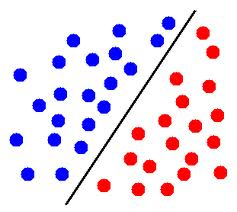
\includegraphics[scale=0.5]{ls}
\end{center}

Shown above is an instance of two-dimensional linear separation. This idea is immediately generalized to n-dimensional Euclidean spaces if the line is replaced by a hyperplane.

\subsection{How is the Perceptron useful here?}
Recall that a Perceptron accepts a set of inputs and produces an output of either 0 or 1. We can pass in the coordinates of each point along with the bias (which we will explain later) and the expected output. This will be a $4x1$ column vector. We will call our input vector $x$. \\

	\begin{center}
		$x = 
		\begin{bmatrix}
			b \\
			i1 \\
			i2 \\
			y
		\end{bmatrix}
		$
	\end{center}

where $b$ is the bias, $i1$ is the x-coordinate of the point, $i2$ the y-coordinate, and $y$ is the expected output (0 or 1). \\

\subsection{Implementing the Perceptron}
We decided to use Python to implement the algorithm. 